\documentclass[12pt]{article}
\usepackage[affil-it]{authblk}
\usepackage{polyglossia}
\usepackage[a4paper,hmargin=3.4cm]{geometry}
\usepackage{mathtools, amssymb, amsfonts}
\usepackage[amsmath]{ntheorem}
\usepackage{fontspec}
\usepackage{titling}
\usepackage{float}
\usepackage{listings}
\usepackage{graphicx}
\usepackage{xcolor}
\usepackage{titling}
\usepackage{tikz}
\usepackage{listings}
\usepackage[hidelinks]{hyperref}
\usepackage{caption,subcaption}
\usepackage{tikz}
\usepackage[locale = FR, exponent-product = \cdot, inter-unit-product = .]{siunitx}
\usetikzlibrary{arrows,shapes,calc,angles,decorations.markings,patterns,decorations.pathmorphing}
\usepackage[shortlabels]{enumitem}
\usepackage{comment}

\setdefaultlanguage{french}
\frenchspacing

\newcommand{\RR}{\mathbb R}
\newcommand{\CC}{\mathbb C}
\newcommand{\QQ}{\mathbb Q}
\newcommand{\ZZ}{\mathbb Z}
\newcommand{\NN}{\mathbb N}
\newcommand{\KK}{\mathbb K}
\newcommand{\FF}{\mathbb F}
\newcommand{\LL}{\mathbb L}
\newcommand{\PP}{\mathbb P}
\newcommand{\EE}{\mathbb E}
\newcommand{\VV}{\mathbb V}

%%%
\theoremstyle{margin}
\theorembodyfont{\normalfont}
\theoremindent0cm
\theoremseparator{:}
\newtheorem{exer}{Exercice}

\theoremstyle{plain}
\theoremindent0.7cm
\newtheorem{ques}{Question}

\theorembodyfont{\itshape}
\newtheorem{prop}{Proposition}


\pretitle{\begin{center}\LARGE
\hrulefill\newline}
\title{{\sffamily Tremplin: Séance 4}}
\posttitle{
\end{center}\vspace{-1em}
\hrulefill}
\date{\today}

\preauthor{\begin{center}}
\author{W. JALLET -- \url{https://github.com/ManifoldFR}}
\postauthor{\end{center}}

\begin{document}
	
\maketitle

\section*{Exercices}

Dans toute la suite, on notera $]a,b[$ l'intervalle \textit{ouvert} d'extrémités $a$ et $b$, qui sont des nombres réels ou $\pm\infty$.

\begin{exer}[\textit{A team of highly trained monkeys}]
Un chimpanzé est assis devant une machine à écrire. La tête d'écriture de la machine défile de gauche à droite, et on considère que le singe la fait se déplacer à gauche avec une probabilité $p\in{]0,1[}$.

On se place dans l'\textit{espace probabilisé} $(\Omega,\mathcal T,\PP)$\footnotemark.
\footnotetext{La notion d'espace probabilisé provient de la théorie classique des probabilités du mathématicien Kolmogorov. $\Omega$ est l'\textit{univers}, $\mathcal T$ est l'ensemble des \textit{évènements}, et $\PP$ est la mesure de probabilité.}

On notera $G$ l'évènement << la tête d'écriture est déplacée à gauche >>, et $R$ l'évènement << la tête d'écriture est déplacée à droite >>. Ainsi, on a avec ces notations
\[ \PP(G) = p.
\]

\begin{enumerate}
\item Quelle est la probabilité $\PP(R)$ que le singe déplace la tête d'écriture à droite?
\end{enumerate}

On va analyser la trajectoire -- aléatoire -- de la tête d'écriture sur le papier. On introduit la famille de variables aléatoires réelles $(X_t)_{t\in \NN}$ sur $\Omega$, telle que $X_t$ correspond à la position de la tête d'écriture à l'instant $t$.

\begin{enumerate}[resume]
\item Soient $t\in\NN$ et $k$ un entier. Quelle est la loi de $X_{t+1}$ conditionnellement à l'évènement $[X_t = k]$ ?
\item Soit $t\in\NN^*$. Quelle est la probabilité que $X_t = k$ en fonction de la loi de $X_{t-1}$.
\end{enumerate}

C'est un peu compliqué. On trouve un système d'équations qui lie la loi de $X_t$ à celle de $X_{t-1}$.\footnote{\textbf{Pour les Spé Maths:} Quand la valeur de $t$ est bornée (disons $t\leq N\in\NN$), on peut réduire le système à un nombre fini d'équations, et le représenter par une matrice dite \textit{stochastique}.}

\begin{figure}[h]
	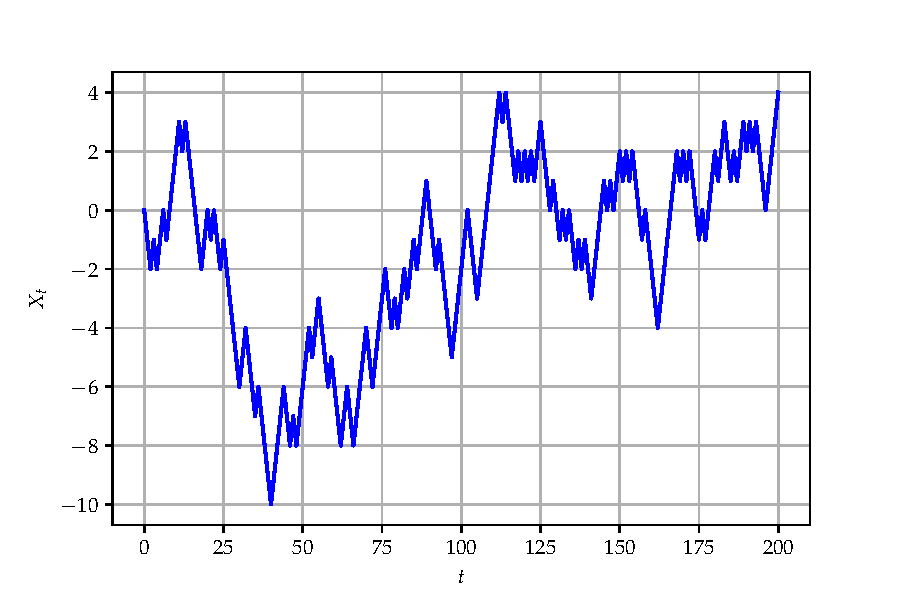
\includegraphics[width=\textwidth]{resources/one_monkey.pdf}
	\caption{Marche aléatoire (\textit{random walk} en anglais) de la tête d'écriture de la machine à écrire.}
\end{figure}

Pour pouvoir calculer l'espérance et la variance de la position $X_t$, on va devoir passer par autre chose. Pour tout $t\geq 0$, on définit le \textit{pas} entre les instants $t-1$ et $t$ par
\[
\xi_t = X_t - X_{t-1}
\]
(On conviendra que $X_{-1} = 0$.)

\begin{enumerate}[resume]
\item Quelle est la loi de $\xi_t$ ?
\item[\textbf{Bonus}] Quelle est la loi de $2\xi_t -1$ ?
\item Justifier que 
\[
\sum_{i=0}^{t}\xi_i = X_t.
\]
\item À quelle condition le singe fait-il, en moyenne, du surplace ? (c'est-à-dire $\EE(X_t) = 0$ pour tout $t$ ?)
\end{enumerate}

Enfin, on va calculer la variance de $X_t$.
\begin{enumerate}[resume]
\item Justifier que les variables $\xi_t$ sont indépendantes.
\item En déduire la variance $\VV(X_t)$.
\end{enumerate}


\vspace{1cm}\textbf{Pour aller plus loin\ldots} Si on met un singe devant une machine à écrire, qui appuie au hasard sur les touches, va-t-il un jour réécrire toute l'œuvre de Shakespeare?


\end{exer}



\end{document}